\documentclass{article}
\usepackage[utf8]{inputenc}
\usepackage{polski}


\usepackage{amssymb, amsmath, amsfonts, amsthm, cite, mathtools, enumerate, rotating, hyperref, enumitem, graphicx, subfig}
\newcommand \eq[1]{\begin{equation} \begin{split}  #1 \end{split} \end{equation}}
\graphicspath{ {../../wykresy/} }

\makeatletter
\newcommand\tab[1][1cm]{\hspace*{#1}}
\def\@seccntformat#1{%
  \expandafter\ifx\csname c@#1\endcsname\c@section\else
  \csname the#1\endcsname\quad
  \fi}
\makeatother

\title{Sprawozdanie do zadania \textbf{P1.11}}
\date{28.10.2020}
\author{Maurycy Borkowski}
\begin{document}
\maketitle
\section{Przedstawienie problemu}
W zadaniu mamy dane mamy równanie zdefiniowane dla $n \geq 2$:
\begin{equation}
\frac{x + x^{-1}}{x^n + x^{-n}} = \frac{1}{n}
\end{equation}
powyższą równość można zapisać równoważnie za pomocą wielomianu $p_n(x)$:
\begin{equation}
p_n(x) = x^n - nx - nx^{-1} + x^{-n}
\end{equation}
równanie ma wtedy postać:
\begin{equation}
p_n(x) = 0
\end{equation}
Wielomian $p_n(x)$ ma ciekawe właściwości:
\newline Ma dokładnie dwa pierwiastki dodatnie: $\alpha$ oraz $\beta$ ($\alpha \in (0,1)$ , $\beta \in (1,3)$), \\dodatkowo ciąg: $\{\beta_n\}^\infty_{n=2}$ jest monotonicznie malejący, to znaczy:
\begin{equation}
\beta_2 > \beta_3 > \ldots > \beta_n
\end{equation}
W zadaniu chcemy znaleźć rozwiązania równania $(1)$ czyli równoważnie pierwiastki $\beta_n$ dla różnych wartości $n \in \{2,3,\ldots 20\}$\\\\
Zauważamy, że znając pierwiastek $\beta_n$ możemy zawęzić zakres poszukiwań pierwiastka $\beta{n+1}$, z (4) $\beta_{n+1} < \beta_{n}$ zatem:
\begin{equation}
\beta_{n+1} \in (1,\beta_n)
\end{equation}
Będziemy ich szukać za pomocą poznanych metod numerycznych szukania miejsc zerowych funkcji, dokładniej:
\begin{enumerate}[label=(\alph*)]
\item metody bisekcji
\item meotdy Newtona
\end{enumerate}
\section{(a) Metoda bisekcji}
Metoda bisekcji opiera swoje działanie na twierdzeniu z analizy rzeczywistej, \href{https://pl.wikipedia.org/wiki/Twierdzenie_Darboux}{Twierdzeniu Darboux}. Podstawowym założeniem tego twierdzenia jest ciągłość badanej funkcji na zadanym przedziale.\\
Łatwo sprawdzić, że tak zdefiniowany (2), wielomian $p_n(x)$ posiada jedyne punkty nieciągłości w $x = 0$. Nie przeszkadza więc nam to w korzystaniu z metody używającej tego twierdzenia, ponieważ ograniczamy się tylko do przedziału występowania pierwiastka $\beta$ tj. podprzedział $(1,3)$.
\newline
Wiemy, że $\beta \in (1,B) \subset (1,3)$ oraz jest to pojedyńczy pierwiastek w tym przedziale, zatem:
\begin{equation}
f(1)f(U) < 0
\end{equation}
Korzystając z Tw. Darboux, (6) oraz $p_n(x)$ jest klasy $C^n$ na przedziale $(1,3)$:
$$
p_n(\beta_n) = 0 \tab dla \tab \beta_n \in (1,3)
$$
Wobec powyższego, możemy zastosować metodę bisekcji do wyznaczenia $\beta_n$.
Dokładny Algorytm metody bisekcji, z którego będziemy korzystać można odnaleźć w książce Analiza Numeryczna, Kincaid David, Cheney Ward (rozdział 3, strona 68).\\\\
Chcemy uzyskać dokładność co najmniej 6 cyfr dziesiętnych tj:
$$
\frac{|r-c_n|}{r} \leq 10^{-6}
$$
dalej (tw. 3.1.2 z Analiza Numeryczna, Kincaid David, Cheney Ward):
$$
2^{-(n+1)} \times \frac{2}{1} = 2^{-n} \leq 10^{-6}
$$
Jest tak dla $n \geq 20$, tyle musimy wykonać iteracji.
\section{(b) Metoda Newtona}
Głównym pomysłem metody Newtona jest przybliżenie badanej funkcji za pomocą \href{https://pl.wikipedia.org/wiki/Wz%C3%B3r_Taylora}{Wzoru Taylora}.
\begin{equation}
0 = f(\beta) = f(x + h) = f(x) + hf^\prime(x) + O(h^2)
\end{equation}
gdzie: 
$h = \beta - x$
Z (7) zauważamy, że aby móc używać korzystać z metody Newtona, $f$ musi być różniczkowalna, oraz $h \lll 1$.\\ W naszym przypadku $f =p_n(x)$ więc pierwsza pochodna istnieje i jest poprawnie określona na całym przedziale występowania $\beta$.\\
Przekształcając (7) mamy, jeżeli $x_n$ jest dobrym przybliżeniem pierwiastka $\beta$ to:
\begin{equation}
x_{n+1} = x_n - \underbrace{\frac{p_n(x_n)}{p_n^\prime(x_n)}}_h
\end{equation}
jest jego lepszym przybliżeniem.\\\\Metoda polega na iterowaniu wzoru (8) i uzyskiwaniu co raz lepszych przybliżeń pierwiastka $\beta$. Dokładny algorytm, z którego będziemy korzysteć można odnaleźć w książce Analiza Numeryczna, Kincaid David, Cheney Ward (rozdział 3, strona 72).\\\\
Widać, że jedynym problemem tej metody jest wyznaczenie \textit{dobrego} $x_0$, bez głębszych i mądrych rozważań na temat własności $p_n(x)$ możemy iterować się po kolejnych wartościach z podprzedziału $(1,3)$ z pewną dokładnością, w ten sposób znajdujemy $x_0$, dla którego metoda będzie szybko zbieżna.\\\\
Liczba iteracji potrzebnych do uzyskania 6 cyfr dziesiętnych dokładności, będzie zależała od wyboru $x_0$.
\section{Implementacja}
Obie metody będziemy implementowali w języku Julia, używając podwójnej precyzji, Float64.
Dla zwiększenia dokładności licząc wartość $p_n(x)$ będziemy używali wzoru (2).\\\\
$p_n(x)^\prime$ potrzebną do metody Newtona wyznaczamy korzystając z podstawowych praw rachunku różniczkowego:
\begin{equation}
p_n(x)^\prime = n ( x^{n-1} + \frac{1}{x^2} - x^{-n - 1} -1)
\end{equation}
\\\\\\\\\\\\\\\\\\\\\\\\\\\\

\section{Wyniki i interpretacja}
Nie będziemy się skupiać na badaniu skuteczności poszczególnych metod z zadania, gdyż problem tego nie dotyczył. Zbadajmy natomiast liczbę iteracji algorytmów poszczególnych metod:

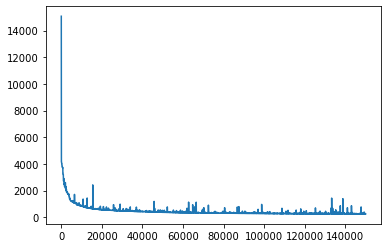
\includegraphics[scale=0.45]{wykres1}

Z powyższego wykresu możemy wywnioskować, że metoda Newtona jest zdecydowanie szybsza dla dowolnych $n$. Metoda bisekcji, nie zmienia (modulo pewna dokładność), ilości iteracji potrzebnych do wyznaczenia $\beta_n$, ponieważ nie powiększamy (a nawet zmniejszamy) zakres poszukiwań.\\
Ilość iteracji w metodzie Newtona spada (też niezbyt znacząco) z powodu lepszego przybliżenia pierwiastka $\beta_n$\\\\
Zbadajmy jak zachowują się kolejne wartości $\beta_n$ wiemy, że maleją (4), ale do czego zbiegają?
\begin{figure}[b!]
  \centering
  \subfloat[Zależność $\beta_n$]{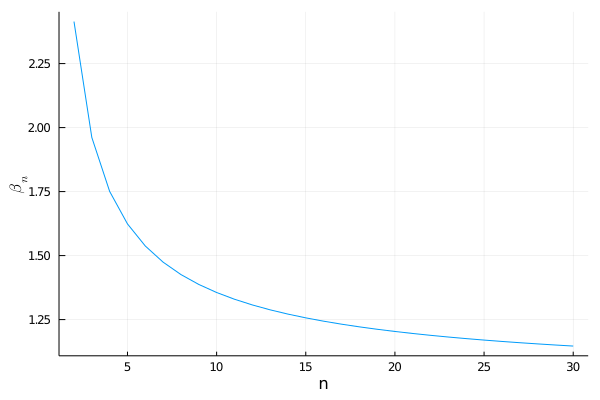
\includegraphics[width=0.5\textwidth]{wykres2}\label{fig:f1}}
  \hfill
  \subfloat[Różnice $\Delta\beta_n$]{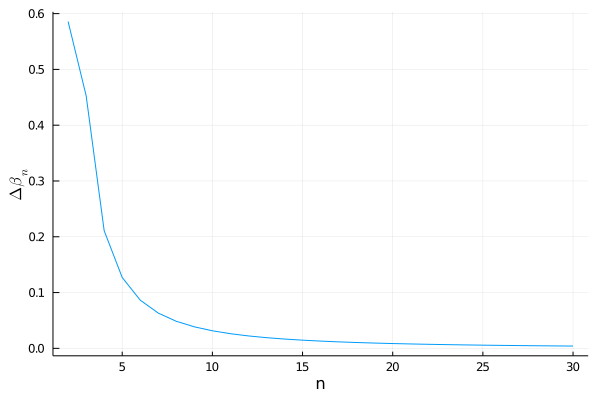
\includegraphics[width=0.5\textwidth]{wykres3}\label{fig:f2}}
\end{figure}
\\\\Z wykresu odczytujemy, że dla $n > 10$ $\beta_n \approx 1.21$ (dokładnie 1.2127491025240678).\\\\
Dla $\pm$ tych wartości $\beta_n$ korekta z (8) $\frac{p_n(x_n)}{p_n^\prime(x_n)}$ jest bardzo mało znacząca przy wzroście $n$ co widać na poniższym wykresie:\\\\

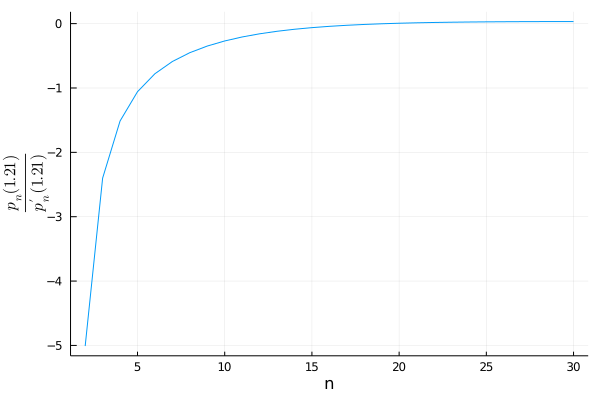
\includegraphics[scale=0.45]{wykres4}

Mimo to metoda Newtona wydaje się być zaskakująco optymalna zestawiona z metodą bisekcji.
\section{Podsumowanie}
Do rozwiązywania problemu poszukiwania rozwiązania równania (1) (równoważnie szukania pierwiastka $p_n(x)$) możemy użyć obu metod, obie dają poprawne rezultaty. Z powyższych rozważań wynika, że optymalniejsze będzie korzystanie z metody Newtona.
% PYTANIA
% Czy musimy profesjonalnie cytować? chcemy?
% Pseudokod na sprawozdaniu?

\end{document}

